\documentclass[10pt]{beamer}
\usetheme{jambro}

\title[]{Pensamento Econômico Contemporâneo - Apresentação}
\author[]{Paulo Victor da Fonseca}
\date{01 de março de 2023}

\hypersetup{
    colorlinks = true,
    urlcolor = teal,
    linkcolor = white    
}
\usepackage[portuguese]{babel}
\usepackage{subfig}
\usepackage{multirow}
\usepackage{engord}
\usepackage{emoji}

\newtheorem{obj}{Objetivo}
\newtheorem{ementa}{Ementa}

\begin{document}

\begin{frame}[plain]
    \titlepage{
        \begin{center}
            \begin{minipage}{0.8\textwidth}
                \centering
            \end{minipage}
        \end{center}}
\end{frame}

\section{Docente}
\begin{frame}{Docente}
    \begin{tabular}{cl}
        \begin{tabular}{c}
            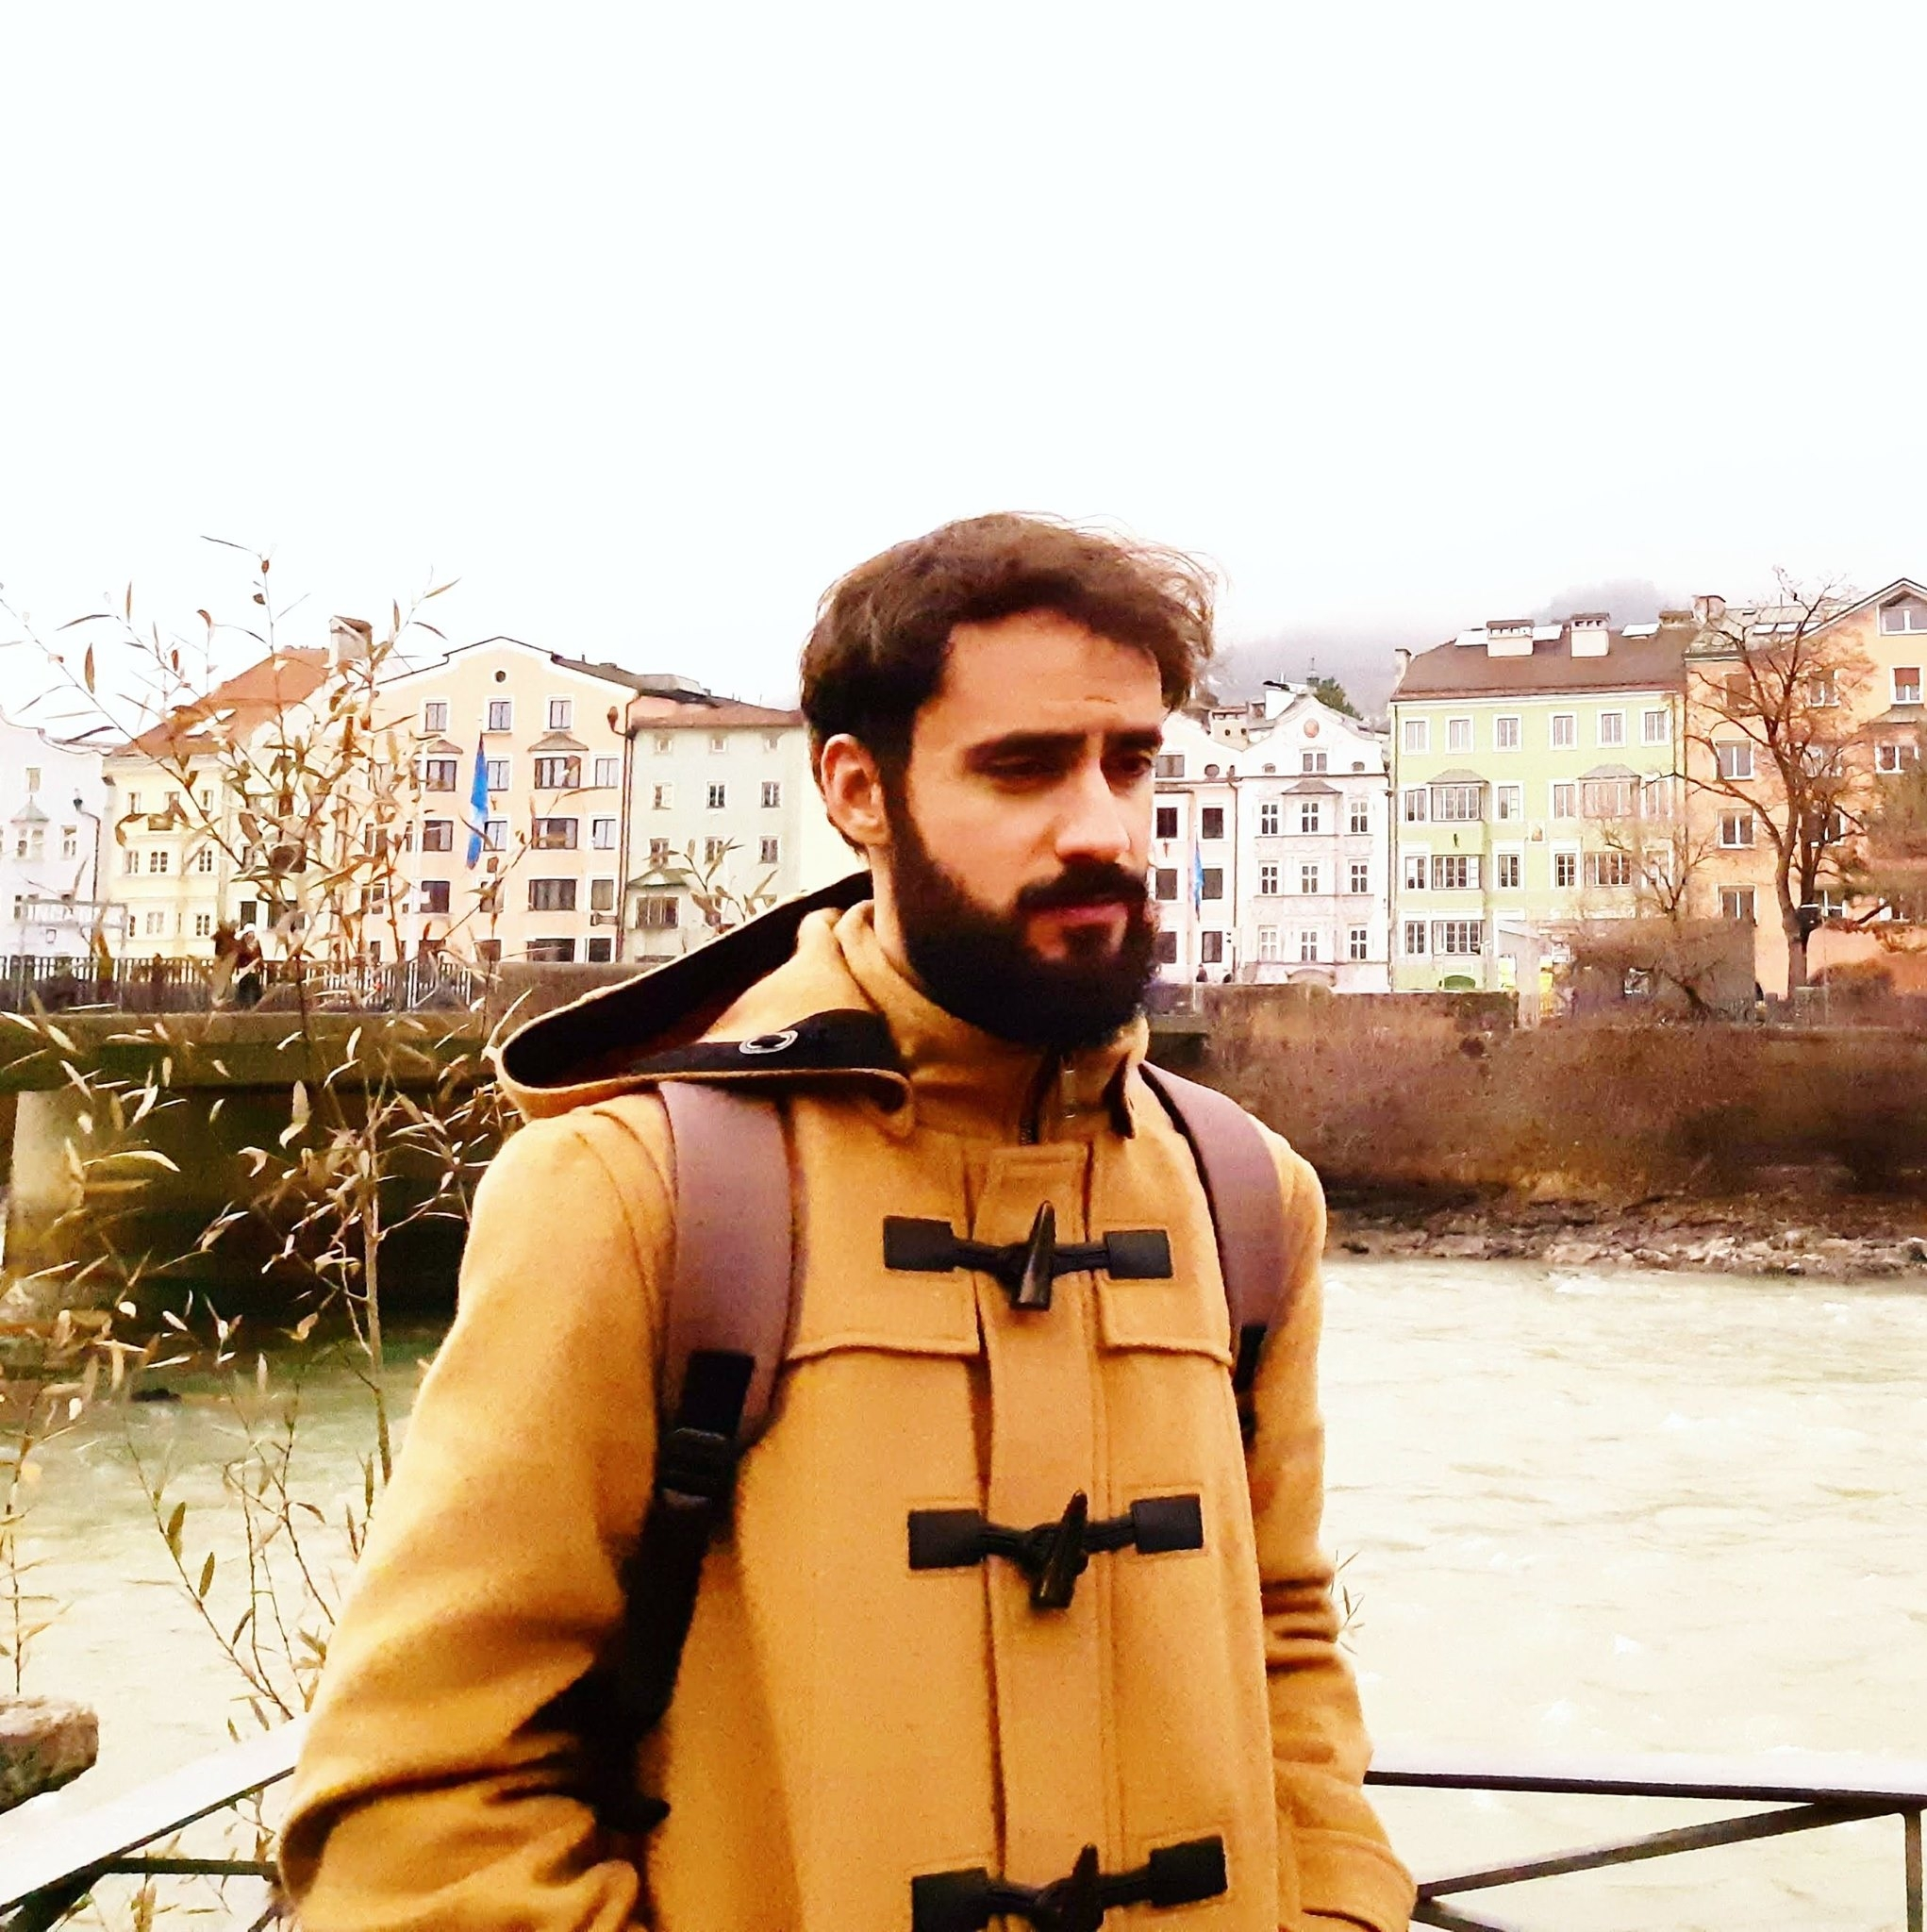
\includegraphics[width=3.5cm]{./figures/Paulo}
        \end{tabular}
         & \begin{tabular}{l}
               \parbox{0.6\linewidth}{
                   \begin{itemize}
                    \item \textbf{Nome:} Paulo Victor da Fonseca\medskip
                    \item \textbf{Formação:} Doutorado em Economia - UFSC\medskip
                    \item \textbf{Áreas de pesquisa:} Macroeconomia. Políticas monetária e fiscal. Modelos DSGE. Modelos novo-Keynesianos com agentes heterogêneos. Modelos baseados em agentes.\medskip
                    \item \textbf{Website:} \href{https://pvfonseca.github.io}{pvfonseca.github.io}\medskip
                    \item \textbf{Contato:} \href{mailto:paulo.fonseca@udesc.br}{paulo.fonseca@udesc.br}
                \end{itemize}
               }
           \end{tabular} \\
    \end{tabular}
\end{frame}

\section{Motivação}
\begin{frame}{Pensamento Econômico Contemporâneo}
    \begin{itemize}
        \item No curso de Pensamento Econômico Contemporâneo, traçaremos a evolução da macroeconomia moderna desde seu início até os dias atuais.\bigskip

        \item Uma justificativa suficiente para esta abordagem é que a macro moderna já existe há tempo suficiente para que valha a pena avaliar os desenvolvimentos da pesquisa macroeconômica nos últimos noventa anos.\bigskip

        \item Uma justificativa adicional é que, durante este período, a macroeconomia passou por uma mudança radical, com a substituição da macroeconomia Keynesiana por modelos dinâmicos e estocásticos introduzidos por Robert Lucas.
    \end{itemize}
\end{frame}

\begin{frame}{Pensamento Econômico Contemporâneo}
    \begin{tabular}{cl}
        \begin{tabular}{c}
            \href{https://www.ineteconomics.org/research/experts/aleijonhufvud}{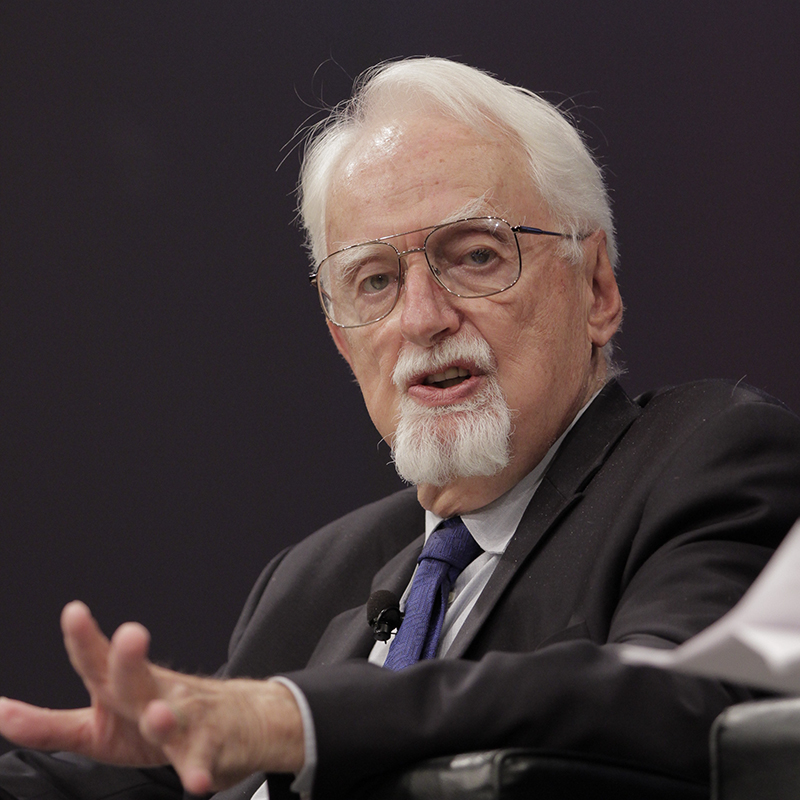
\includegraphics[width=3.5cm]{./figures/axel.jpg}}
        \end{tabular}
         & \begin{tabular}{l}
               \parbox{0.6\linewidth}{
                \begin{minipage}{.7\textwidth}
                    \NB{``O principal objetivo da história do pensamento econômico da segunda metade do século XX é, seguramente, explicar esta mudança de 180 graus na visão de mundo do (macro)economista representativo.'' \\
                        \begin{flushright}
                            (Leijonhufvud, 2006 - Episodes in a century of Macroeconomics).
                        \end{flushright}}
                \end{minipage}
               }
           \end{tabular} \\
    \end{tabular}    
\end{frame}

\begin{frame}{Pensamento Econômico Contemporâneo}
    \begin{itemize}
        \item Dois eventos importantes são identificáveis na história da macroeconomia moderna:\medskip
              \begin{enumerate}
                  \item A transição do que foi escrito por Keynes na `Teoria Geral' para o que se tornou a macroeconomia nas mãos dos economistas Keynesianos - a transição da `Economia de Keynes' para a `Economia Keynesiana'.\medskip

                  \item A revolução iniciada por Robert Lucas, que destronou a macroeconomia Keynesiana.
              \end{enumerate}
    \end{itemize}
\end{frame}

\begin{frame}{Pensamento Econômico Contemporâneo}
    \begin{itemize}
        \item Portanto, colocando de lado a Teoria Geral de Keynes, a história da macroeconomia moderna pode ser dividida em duas eras:\medskip

              \begin{enumerate}
                  \item 1940s - 1970s: dominância da macroeconomia Keynesiana.\medskip

                  \item 1970s - presente: era da macroeconomia dos modelos DSGE (paradigma dominante nos dias atuais).
              \end{enumerate}
    \end{itemize}
\end{frame}

\begin{frame}{Pensamento Econômico Contemporâneo}
    \begin{center}
        \begin{minipage}{.8\textwidth}
            \NB{Grandes economistas forçam seus contemporâneos a fazerem escolhas - o que perguntar, o que assumir, o que considerar como evidência, e quais métodos e modelos utilizar - e persuadem a profissão ou uma fração dela a adotar as escolhas que fizeram. A trajetória que qualquer escola de pensamento particular adotou acompanha tais decisões. Muitas das escolhas tomadas em uma sequência como esta não foram antecipadas pelo fundador ao qual traçamos o desenvolvimento em questão mas, sim, foram adotadas pelos contribuintes subsequentes; algumas das decisões tomadas podem ser consideradas erradas quando avaliadas em retrospectiva. \\
                \begin{flushright}
                    (Leijonhufvud, 1994 - Hicks, Keynes and Marshall).
                \end{flushright}}
        \end{minipage}
    \end{center}
\end{frame}

\begin{frame}[plain]{Apresentação: 83PEC - Pensamento Econômico Contemporâneo}
    \begin{figure}
        \centering
        \hspace*{-9mm}
        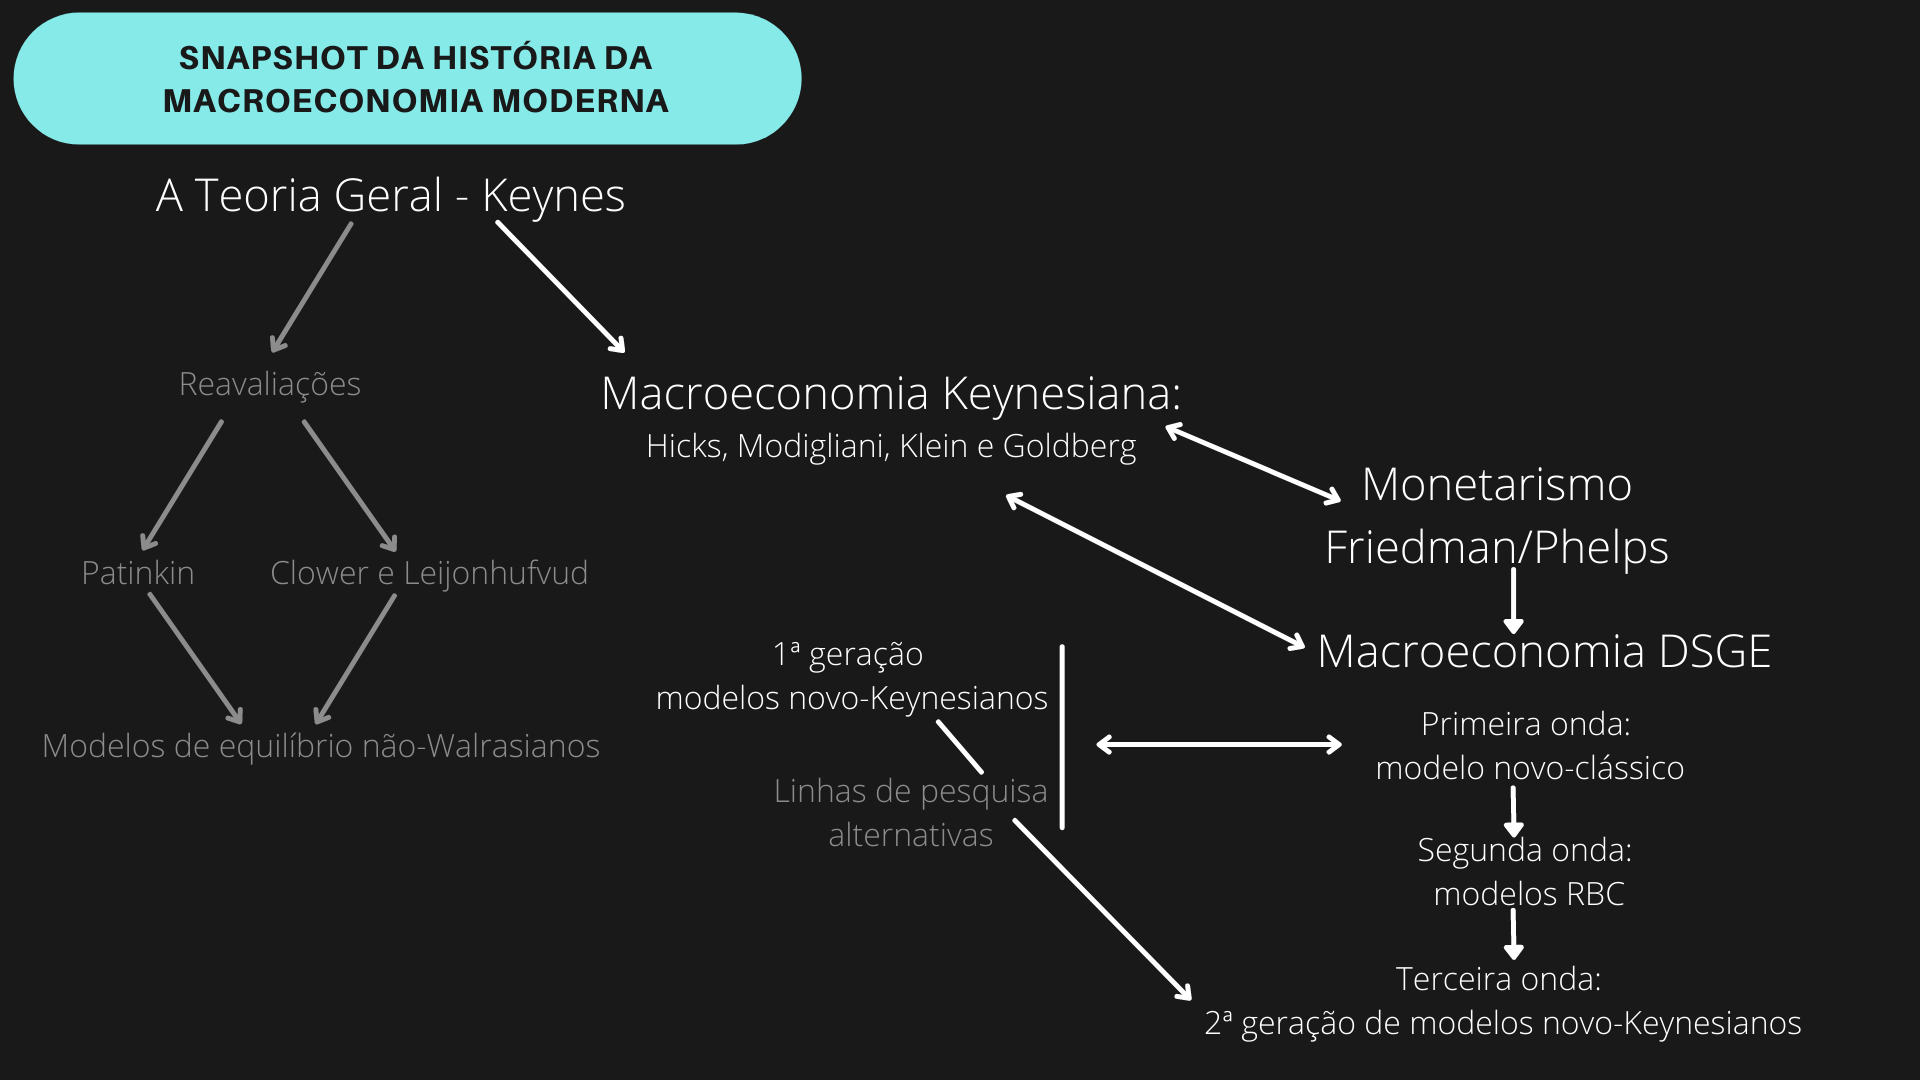
\includegraphics[width=.8\textwidth]{./figures/snapchot}
        \caption{Snapshot da história da macroeconomia moderna. Fonte: De Vroey (2016).}
        \label{fig.snap}
    \end{figure}
\end{frame}

\begin{frame}{Pensamento Econômico Contemporâneo}
    \begin{center}
        \footnotesize
        \begin{tabular}{l l}
            \hline
            \textbf{Episódio}                                                                                    & \textbf{Referências}                            \\
            \hline
            \hline
            \hlight{Teoria Geral do Emprego, do Juro e da Moeda}                                                 & Keynes                                          \\
            \hlight{Macroeconomia Keynesiana (IS-LM)}                                                            & Hicks, Modigliani, Klein                        \\
            \hlight{Monetarismo}                                                                                 & Friedman                                        \\
            \hlight{Taxa natural de desemprego}                                                                  & Friedman, Phelps                                \\
            Teoria de desequilíbrio                                                                              & Patinkin, Clower e Leijonhufvud                 \\
            Modelos de equilíbrio não-Walrasianos                                                                & Barro e Grossman, Benassi, Drèze, Malinvaud     \\
            \hlight{DSGE I: macroeconomia Lucasiana}                                                                                                               \\ \quad \hlight{(novos-cl\'{a}ssicos ou revolu\c{c}\~{a}o das} \\ \quad \hlight{expectativas racionais)} & Lucas, Sargent, Wallace, Barro \\
            \multirow{2}{*}{\hlight{1\textsuperscript{a} gera\c{c}\~{a}o de modelos novo-Keynesianos}}           & Akerlof, Azariadis, Ball, Blanchard, Fischer,   \\ & Mankiw, Romer, Shapiro e Stiglitz, Solow, Taylor \\
            Linhas de pesquisa alternativas                                                                      & Carlin e Soskice, Diamond, Hart, Roberts        \\
            \hlight{DSGE II: modelos RBC}                                                                        & Kydland e Prescott                              \\
            \multirow{2}{*}{\hlight{DSGE III: 2\textsuperscript{a} gera\c{c}\~{a}o de modelos novo-Keynesianos}} & Blanchard, Christiano, Eichenbaum e Evans, Gali \\ & Taylor, Rotemberg, Smets e Wouters, Woodford \\
            \hline
        \end{tabular}
    \end{center}
\end{frame}



\begin{frame}{Pensamento Econômico Contemporâneo}
    A disciplina 83PEC - Pensamento Econômico Contemporâneo aborda as principais correntes do pensamento econômico contemporâneo, enfatizando seu desenvolvimento em contextos históricos e analisando as contribuições metodológicas ao pensamento atual. O curso é dividido em sete blocos:\medskip

    \begin{enumerate}
        \item Introdução: modelo clássico vs. Keynes\medskip

        \item Síntese neoclássica\medskip

        \item O pensamento de Milton Friedman e a escola monetarista\medskip

        \item A escola novo-clássica\medskip

        \item Ciclos reais de negócios\medskip

        \item Novos-Keynesianos e o novo consenso macroeconômico\medskip

        \item Teorias do crescimento econômico
    \end{enumerate}
\end{frame}

\section{Ementa}
\begin{frame}{Pensamento Econômico Contemporâneo: Ementa}
    \begin{center}
        \begin{minipage}{.8\textwidth}
            \NB{O Pensamento Econômico de Milton Friedman. A Síntese Neoclássica. \\ Novos Clássicos. Novos Keynesianos. Ciclos Reais. \\ Nova Teoria do Crescimento. Novo Consenso.}
        \end{minipage}
    \end{center}
\end{frame}

\section{Objetivo}
\begin{frame}{Pensamento Econômico Contemporâneo: Objetivo}
    \begin{center}
        \begin{minipage}{.8\textwidth}
            \NB{O objetivo da disciplina é abordar as principais correntes do pensamento econômico contemporâneo, enfatizando seu desenvolvimento em \\ contextos históricos com problemáticas específicas e analisando as \\ contribuições metodológicas destas escolas ao pensamento atual.}
        \end{minipage}
    \end{center}
\end{frame}

\section{Formato das aulas e sistema de avaliação}
\begin{frame}{Formato das aulas e sistema de avaliação}
    \begin{itemize}
        \item A disciplina apoia-se, fundamentalmente, em livros-texto e notas de aula e será ministrada por meio de aulas expositivas.\bigskip

        \item As aulas acontecerão às:\medskip
              \begin{itemize}
                  \item Quartas-feiras das 08:20 às 10:00.\medskip
                  \item Sextas-feiras das 08:20 às 10:00.\bigskip
              \end{itemize}

        \item A avaliação será realizada a partir dos procedimentos abaixo:\medskip
              \begin{itemize}
                  \item Atividade avaliativa I (PI): 20\%\medskip
                  \item Atividade avaliativa II (PII): 30\%\medskip
                  \item Atividade avaliativa III (PIII): 30\%\medskip
                  \item Trabalhos adicionais: 20\%
              \end{itemize}
    \end{itemize}
\end{frame}

\begin{frame}{Formato das aulas e sistema de avaliação}
    \begin{itemize}
        \item Os alunos devem ter em mente que o aprendizado e o acompanhamento do curso dependem essencialmente de seu próprio esforço.\bigskip

        \item Os tópicos do programa serão apresentados em aulas expositivas, destinadas à apresentação de conceitos, modelos e suas aplicações.\bigskip

        \item[\emoji{warning}] \hlight{Embora importantes, as aulas n\~{a}o podem jamais ser vistas como substitutas da leitura regular e cuidadosa dos textos indicados e da resolu\c{c}\~{a}o dos exerc\'{i}cios propostos.}
    \end{itemize}
\end{frame}

\section{Bibliografia}
\begin{frame}{Bibliografia}
    \begin{figure}
        \centering
        \subfloat[Snowdon e Vane (2005)\label{fig2b}]{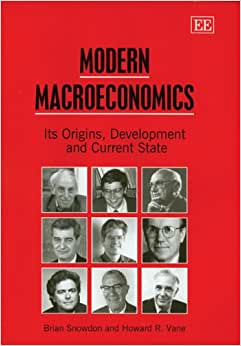
\includegraphics[width=0.21\textwidth]{./figures/snowdon}} \qquad
        \subfloat[De Vroey (2016)\label{fig2a}]{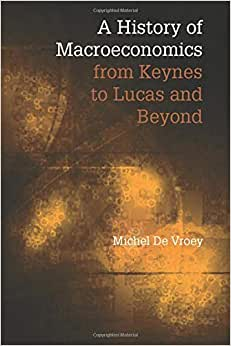
\includegraphics[width=0.2\textwidth]{./figures/devroey}} \qquad
        \subfloat[Blanchard (2017)\label{fig2c}]{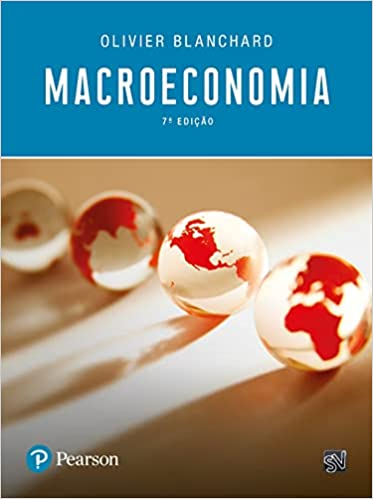
\includegraphics[width=0.22\textwidth]{./figures/blanchard}}
        \caption{Bibliografia do curso}
        \label{fig2}
    \end{figure}
\end{frame}

\begin{frame}{Bibliografia}
    \begin{figure}
        \centering
        \subfloat[Froyen (2013)\label{fig1b}]{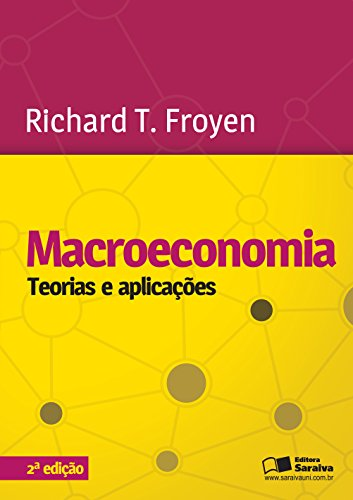
\includegraphics[width=0.22\textwidth]{./figures/froyen}} \qquad
        \subfloat[Romer (2018)\label{fig1c}]{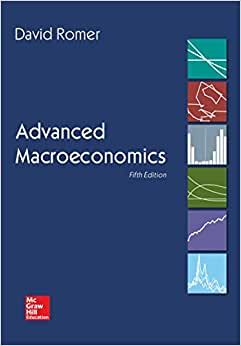
\includegraphics[width=0.22\textwidth]{./figures/romer}} \qquad
        \subfloat[Jones e Vollarth (2014)\label{fig3c}]{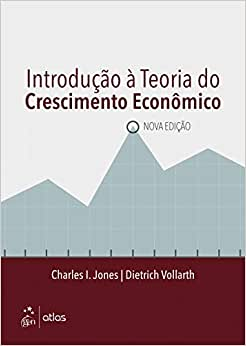
\includegraphics[width=0.22\textwidth]{./figures/jones}}
        \caption{Bibliografia do curso}
        \label{fig1}
    \end{figure}
\end{frame}

\begin{frame}{Bibliografia}
    \begin{itemize}
        \item BLANCHARD, O. \emph{Macroeconomia}. 7.ed. São Paulo: Pearson Education do Brasil, 2017.\medskip
        \item DE VROEY, M. \emph{A History of Macroeconomics from Keynes to Lucas and Beyond}. Cambridge University Press, 2016.\medskip
        \item FROYEN, R. \emph{Macroeconomia: teorias e aplicações}. 2.ed. São Paulo: Saraiva, 2013. Disponível em: \href{https://app.minhabiblioteca.com.br/books/9788502175235}{app.minhabiblioteca.com.br/books/9788502175235}\medskip
        \item JONES, C.I. \emph{Introdução à Teoria do Crescimento Econômico}. São Paulo: Campus, 2000.\medskip
        \item ROMER, D. \emph{Advanced Macroeconomics}. 4.ed. Boston, MA: McGraw-Hill, 2012.\medskip
        \item SNOWDON, B.; VANE, H.R. \emph{Modern Macroeconomics: its Origins, Development and Current State}. Northampton, MA: Edward Elgar, 2005.
    \end{itemize}
\end{frame}
\end{document}